\documentclass[../main.tex]{subfiles}
\begin{document}
Chapter~\ref{chapter:intro} established the foundational context by identifying the innovation deadlock faced by SMEs, defining research aims for affordable person Re-ID systems, and outlining the thesis contributions. This chapter presents related works in Section~\ref{sec:related} and foundation theory in Section~\ref{sec:foundtheo}, where models, frameworks, and algorithms for the end-to-end pipeline are detailed. To achieve the thesis objectives, four key technical components are examined: lightweight object detection using YOLOv11 for CPU-based edge deployment (Section~\ref{sec:objdect}), efficient object tracking through ByteTrack algorithms (Section~\ref{sec:objtrack}), optimized feature extraction and lightweight image classification for human metadata in limited hardware resource (Sections~\ref{sec:feature_extraction} and~\ref{sec:image_classification}), and distributed system infrastructure including message queuing,\\ containerization, and vector database optimization (Sections~\ref{sec:message_queue},~\ref{sec:containerization}, and~\ref{sec:vector_database}).

\section{Related works}
\label{sec:related}

\subsection{Person Re-Identification}
\label{sec:personreid}

Recent advances in person Re-ID have significantly enhanced performance across various scenario, primarily relying on powerful computational resources. In the context of visible–infrared ReID, Guo et al. (2025) introduced the Region‑based Augmentation and Cross Modality Attention (RACA) model \cite{visible-infrared-reid}, which leverages region-level augmentation (PedMix) and a modality feature transfer (MFT) module with cross-attention to reduce interference between modalities, yielding notable improvements on SYSU‑MM01 and RegDB benchmarks.

Addressing unsupervised learning, Qin et al. (2025) proposed Attention‑based Hybrid Contrastive Learning (AHCL) \cite{unsupervised-reid}. Their framework integrates spatial and channel attention with a hybrid contrastive loss, combining cluster-level and instance-level representations to bolster ReID accuracy without labels.
 
Multimodal ReID has been further advanced by Yan et al. (2025) through \\ FusionSegReID \cite{fusionsegreid}, which fuses image features, textual descriptions, and \\ segmentation masks to enhance robustness—especially in occluded or low-quality scenarios. Interactive, language-driven retrieval was pushed forward by Niu et al. (2025) in ChatReID \cite{chatreid}. This framework uses a Vision–Language Model (LVLM) with Hierarchical Progressive Tuning, enabling interactive, VQA-style queries to improve identity-level matching performance.

Despite the impressive progress of person ReID, most state-of-the-art models demand substantial hardware and computational resources, limiting their practicality on lightweight or embedded devices. To address this, \textbf{OSNet} (Omni-Scale Network) was proposed by Zhou et al.~\cite{zhou2019omniscalefeaturelearningperson}. OSNet is a compact yet powerful architecture, specifically designed for efficient deployment. It employs \textit{omni-scale feature learning}, utilizing multiple convolutional streams with varying receptive field sizes within each residual block to capture both fine-grained details and global features. Additionally, OSNet integrates a \textit{Unified Aggregation Gate (UAG)} that adaptively fuses multi-scale features via channel-wise weighting. By leveraging depthwise-separable convolutions, OSNet significantly reduces computational cost and model size, achieving state-of-the-art performance despite being substantially lighter than standard models like ResNet-50.

Building upon OSNet's efficiency, \textbf{LightMBN} (Lightweight Multi-Branch Network) introduced by Herzog et al.~\cite{Herzog_2021} further optimizes this backbone architecture. LightMBN expands OSNet by adding specialized global, part-based, and channel-wise branches, thereby enriching feature representations without significant complexity increases. It also incorporates enhanced training techniques, including label smoothing, random erasing, and cosine learning rate schedules, leading to improved generalization performance. Consequently, LightMBN achieves impressive accuracies on widely-used benchmarks like Market-1501 and CUHK03, outperforming many heavier architectures while remaining lightweight and suitable for resource-constrained deployments.

Given their complementary strengths in efficiency and performance, OSNet and LightMBN form a robust backbone choice for deployment in lightweight Re-ID pipelines.


\subsection{Edge Computing in AI}
\label{sec:edgecomputing}

Edge computing has emerged as a transformative approach in artificial intelligence, bringing computational resources closer to where data is generated and directly to end users. The global edge AI market size was valued at approximately USD 20.78 billion in 2024 and is expected to grow significantly, at a rate of 21.7\% annually, from 2025 to 2030 \cite{grandview2024}. This growth indicates a strong demand for real-time processing, lower latency, and improved privacy in various AI applications.

Within retail and customer experience contexts, edge computing provides substantial benefits. It enables retail IT teams to manage cloud expenses effectively by strategically selecting which data to send to the cloud, processing only critical information rather than all raw data \cite{biztech2024}. This selective processing is particularly beneficial for person Re-ID systems, where enormous video data streams can be filtered and analyzed locally, and only essential features are transmitted to centralized servers.

Recent research has also concentrated on adapting AI models specifically for edge environments. Novel person Re-ID methods incorporate pedestrian edge features directly into their representations and leverage these edge characteristics to enhance global context feature extraction \cite{mdpi2024_edge}. Such methods highlight the practical feasibility of deploying sophisticated Re-ID algorithms on devices with limited computational capabilities.

Edge AI is becoming more widely available across many applications. Edge Intelligence, or Edge AI, means moving AI processing from cloud systems directly to edge devices where data is created. This change is important for making AI more available and affordable, especially for organizations that may find cloud-based AI solutions too expensive \cite{viso2024}.

Therefore, this thesis leverages edge computing paradigms to distribute computational workloads across edge devices, enabling cost-effective deployment of person Re-ID systems while maintaining real-time performance requirements.

\subsection{Microservices and Distributed Systems}
\label{sec:microservice}

Microservices have become increasingly popular for building scalable AI systems. In general, microservices focus on modularity, meaning each service handles a specific function independently. These services are loosely connected, easy to deploy individually, and can scale separately \cite{wiki2024_microservices}.

In person Re-ID systems, microservices offer clear advantages, especially when deployed across distributed environments. For example, using microservices in combination with AI-powered edge computing gateways helps handle privacy concerns while efficiently identifying the same person from multiple camera angles and locations \cite{mdpi2021_microservice}.

However, using distributed setups in Re-ID introduces new challenges. Traditional Re-ID algorithms typically prioritize accuracy but aren't designed with distributed deployment in mind. Distributed environments demand algorithms that are lightweight and computationally efficient \cite{ieee2015_distributed}. Thus, there is a significant need for simpler, more efficient Re-ID algorithms suitable for running on multiple edge nodes.

Recent studies have explored distributed frameworks for deep learning applications, particularly using microservices for object detection tasks on edge devices. These frameworks effectively analyze images and videos to extract relevant object information and locations, providing a solid foundation for scalable Re-ID applications involving many cameras or geographic areas \cite{mdpi2023_framework}.

Cloud-based solutions have also been investigated. Video-based person Re-ID using distributed cloud computing stores pedestrian data and model parameters across multiple cloud servers to improve reliability and reduce failures \cite{jait2022_cloud}. However, ongoing cloud service costs can be prohibitive for small and medium-sized businesses.

Introducing a message broker into a microservices architecture provides additional advantages. Message brokers enable seamless communication among microservices by handling data exchange, enhancing reliability, and simplifying integration. Specifically, they help Re-ID systems quickly share person-related data across various cameras and processing units, ensuring low latency and better system scalability.

Overall, the shift toward microservices architecture, combined with the use of message brokers, reflects a broader trend towards modular, scalable, and efficient AI system deployment, making it particularly beneficial for distributed person Re-ID solutions in retail and similar settings \cite{splunk2024}. To maximize the performance of the system by avoiding bottlenecks in any components of the centralized server, this thesis utilizes a microservices architecture to distribute the computational workload across edge devices and the central server.


\section{Foundation theory}
\label{sec:foundtheo}

\subsection{Object detection}
\label{sec:objdect}

Object detection technology finds applications across numerous domains including automatic traffic violation systems, identification of unfamiliar persons, digital attendance systems, and autonomous robotic vehicles. The advent of deep learning has dramatically enhanced object detection capabilities. Region-Based Convolutional Neural Networks (R-CNN) \cite{girshick2014richfeaturehierarchiesaccurate} represented one of the pioneering breakthroughs in this area, combining CNN architectures \cite{oshea2015introductionconvolutionalneuralnetworks} with region proposal mechanisms to achieve accurate object localization and classification in images. Subsequent iterations, Fast R-CNN \cite{girshick2015fastrcnn} and Faster R-CNN \cite{ren2016fasterrcnnrealtimeobject}, were developed to enhance both processing speed and detection precision compared to the original model. Despite these improvements in detection performance, the multi-step processing pipeline made these approaches impractical for real-time applications.

Modern frameworks such as Detectron2 \cite{Merz_2023} and EfficientDet \cite{tan2020efficientdetscalableefficientobject} have pushed object detection forward considerably. Detectron2 offers flexible deployment of high-performing models but demands extensive setup and typically involves \\computationally heavy architectures, making it unsuitable for real-time or resource-limited environments. EfficientDet provides a more practical option for devices with constrained resources, though it may struggle to meet strict real-time performance criteria.

You Only Look Once (YOLO) addresses the limitations of multi-stage detection approaches by reformulating object detection as a single regression problem. YOLO processes the entire image in one forward pass, directly predicting bounding boxes and class probabilities from full images. This unified architecture enables real-time performance while maintaining reasonable accuracy for many applications.

The YOLO family has evolved through multiple iterations, with each version improving upon speed-accuracy trade-offs. YOLOv11 \cite{khanam2024yolov11overviewkeyarchitectural}, in particular, offers several model variants ranging from nano (yolo11n) to extra-large (yolo11x)\\configurations. The nano variant is specifically designed for resource-constrained environments, featuring significantly reduced parameters and computational requirements while preserving essential detection capabilities.

\begin{figure}[h!]
\centering
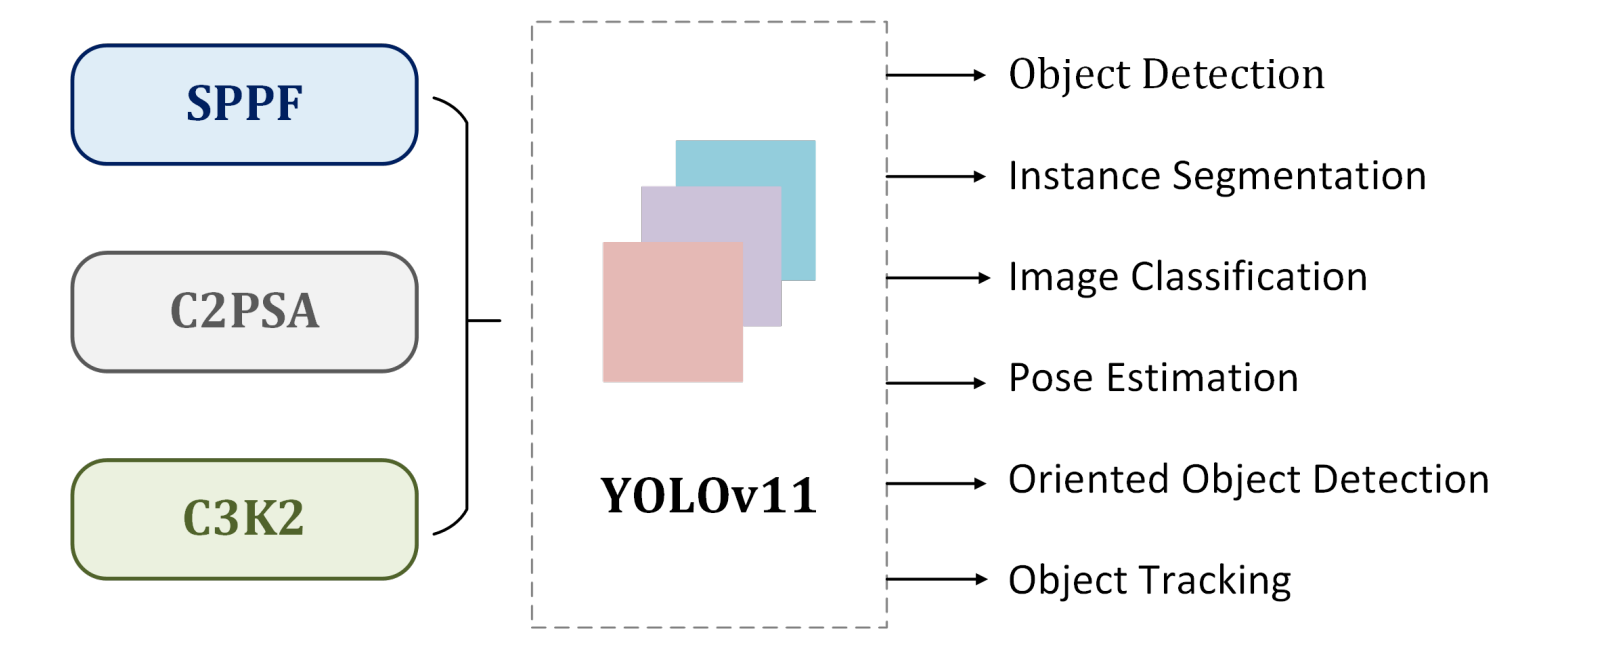
\includegraphics[width=\linewidth]{Figure/yolov11.png}
\caption{ Key architectural modules in YOLO11~\cite{khanam2024yolov11overviewkeyarchitectural}.}
\label{fig:yolov11}
\end{figure}

A significant advancement in YOLOv11 is the integration of thhe C2PSA \\(Convolutional
block with Parallel Spatial Attention) component, which enhances spatial attention capabilities beyond previous YOLO iterations. The C2PSA block enables the model to focus more effectively on critical regions within images by inaplementing parallel spatial
attention mechanisms. This enhancement is particularly beneficial for detecting objects of varying sizes and positions, addressing common challengees in complex visual environments with partially occluded or small objects. The retention of the Spatial Pyramid Pooling - Fast (SPPF) blockfrom previous versions, combined with the new C2PSA component, creates a compreehensive feature processing pipeline that balances computational efficiency with enhancced spatial awareness.

For edge-based human monitoring applications, YOLOv11n provides an optimal balance between detection performance and computational efficiency. Its lightweight architecture enables deployment on edge devices for real-time person detection, serving as the foundation for subsequent tracking and Re-ID processes in distributed camera networks.

\subsection{Object tracking}
\label{sec:objtrack}

Person Re-ID systems face significant challenges when relying solely on frame-by-frame analysis. Individuals frequently lose their visual identity due to various factors including occlusions from other people or objects, rapid movement causing motion blur, and temporary disappearance from camera coverage areas. While deep learning-based feature extraction models can effectively capture contextual information and compute discriminative identity embeddings, frame-based matching approaches often suffer from identity fragmentation—where the same person receives multiple different identities across consecutive frames.

To address these limitations, tracking mechanisms play a crucial role in maintaining identity consistency over temporal sequences. Unlike existing methods that perform Re-ID independently for each frame, tracking-based approaches maintain continuous identity associations across time. This temporal continuity significantly outperforms computationally expensive alternatives such as query-driven region proposals \cite{munjal2019queryguidedendtoendpersonsearch} and graph-based retrieval methods \cite{zhu2025graphbasedapproachesfunctionalitiesretrievalaugmented}, which become prohibitively costly in large-scale deployment scenarios. By leveraging tracking, our system can efficiently associate multiple detections of the same person, substantially reducing redundant identity searches while improving real-time processing capabilities.

The development of multi-object tracking (MOT) algorithms has evolved through several generations, each addressing specific limitations of previous approaches. 

Multi-object tracking has evolved through several approaches, each with distinct trade-offs. SORT \cite{sort} provides efficient tracking by integrating object detection with motion prediction, but struggles with complex movement patterns and fast-paced scenarios. To address these limitations, DeepSORT \cite{deepsort} incorporates appearance features via a pre-trained Siamese network, improving performance in dense environments where motion alone is inadequate. However, this enhancement introduces dependency on embedding quality and computational complexity, making it susceptible to visual disturbances. FairMOT \cite{fairmot} advances this paradigm by merging detection and tracking into a unified architecture that simultaneously produces detection outputs and Re-ID features for enhanced multi-object tracking. This unified approach, while effective, demands significant computational resources and requires careful optimization between detection and Re-ID objectives, ultimately compromising processing speed. Alternative solutions include MMTracking \cite{mmtracking}, which provides a versatile framework supporting multiple advanced algorithms but necessitates substantial parameter optimization.

ByteTrack \cite{bytetrack} represents a breakthrough in tracking methodology, delivering exceptional performance without requiring dedicated appearance models, thereby maintaining high processing speeds particularly in crowded environments. This approach achieves an optimal trade-off between real-time processing and tracking reliability. Consequently, our framework employs ByteTrack for maintaining pedestrian identity consistency across video frames, significantly enhancing ID assignment precision. This capability proves essential in dense scenarios where overlapping persons create significant challenges for camera-based identification systems.

\subsection{Feature extraction}
\label{sec:feature_extraction}

Feature extraction serves as the cornerstone of person Re-ID systems, transforming raw image data into compact descriptors suitable for robust identity matching. To enhance efficiency, especially for deployment on resource-constrained edge devices, recent research has focused on designing specialized lightweight feature extraction architectures.

For instance, Wang et al.~introduced the Attention Knowledge-distilled Lightweight Network (ADLN) \cite{adln}, specifically tailored for edge applications. ADLN utilizes a dimension interaction attention module to improve channel-wise feature representation, complemented by self-distillation that transfers learned attention patterns from deeper layers to shallower ones. Employing a combination of cross-entropy, weighted triplet, and center loss, ADLN effectively minimizes intra-class variability, achieving competitive accuracy on widely-used benchmarks such as Market-1501 and DukeMTMC-ReID, while significantly reducing computational complexity.

Building on similar objectives, Gao et al.~presented a joint attention-based Re-ID model \cite{jointattention}. This model emphasizes both global and local pedestrian features through integrated attention modules, achieving precise and discriminative feature extraction that aligns well with realistic surveillance scenarios. This balance between accuracy and computational efficiency makes the model highly suitable for edge deployment.

Recent advances have also explored lightweight Transformer-based architectures, notably LightAMViT~\cite{lightamvit}. By streamlining self-attention mechanisms through K-means-based token clustering and adaptive weighted pooling, LightAMViT significantly reduces computational demands compared to traditional Vision Transformers. This approach provides a practical alternative, blending the strong representational capability of Transformers with the computational efficiency required by edge devices.

Complementing these specialized architectures, broader efforts in mobile-optimized methodologies such as MobileNetV2 \cite{sandler2019mobilenetv2invertedresidualslinear} and MobileNetV3 \cite{howard2019searchingmobilenetv3} have gained prominence in edge-based AI applications. These networks use depth-wise separable convolutions to significantly cut down computational overhead while preserving accuracy. Additionally, Squeeze-and-Excitation Networks (SE-Net) \cite{hu2019squeezeandexcitationnetworks} introduce adaptive channel-wise recalibration mechanisms, further enhancing model efficiency by focusing computation on informative image regions.

However, despite these general improvements, generic lightweight architectures often lack specific optimizations required by the complexities of person Re-ID tasks. This gap has motivated dedicated research into architectures explicitly designed for Re-ID applications.

Among these specialized designs, OSNet (Omni-Scale Network) \cite{zhou2019omniscalefeaturelearningperson} represents a significant advancement. With only 2.2 million parameters, OSNet is substantially smaller than traditional methods like ResNet-50, which typically use around 24 million parameters, making it highly suitable for edge deployment. OSNet introduces innovative omni-scale feature learning through a novel building-block design, effectively capturing multi-scale information without the heavy computational cost typically associated with traditional multi-scale approaches. Its use of depth-wise separable convolutions and channel-shuffling operations maintains computational efficiency while preserving strong discriminative capability.

Expanding on OSNet's approach, LightMBN (Lightweight Multi-Branch Network) \cite{Herzog_2021} further advances edge-friendly Re-ID through a multi-branch design tailored for constrained environments. LightMBN integrates efficient channel-wise and spatial attention mechanisms, adaptively emphasizing informative features without significantly increasing computational load. This enables robust identity matching with minimal resource usage.

\subsection{Image classification}
\label{sec:image_classification}

Traditionally, image classification and person Re-ID have been considered distinct tasks, with limited overlap. Person Re-ID focuses on matching individuals across different camera views, while image classification typically identifies broad object categories. However, when considering scenarios with a large search space—potentially thousands of identities—performing direct identity matching can be computationally expensive and slow. Under these conditions, reducing the search space using easily classifiable human metadata, such as gender, becomes beneficial by limiting the number of candidates considered, thus improving retrieval speed and accuracy.

Commonly used image classification models include well-established convolutional neural networks (CNNs) such as ResNet~\cite{he2015deepresiduallearningimage}, known for its deep residual learning framework that significantly improves accuracy in classification tasks. MobileNet~\cite{mobilenet} offers lightweight architectures optimized for resource-constrained devices, leveraging depth-wise separable convolutions to reduce computational costs. More recently, Vision Transformers (ViT)~\cite{ViT} have introduced transformer-based architectures to image classification, leveraging self-attention mechanisms to capture global relationships, achieving impressive accuracy at the cost of higher computational demands.

To effectively balance accuracy and computational efficiency in edge-based systems, EfficientNet~\cite{efficientnet} was introduced. EfficientNet leverages a compound scaling method to optimally adjust network depth, width, and resolution. Among its variants, EfficientNet-B0 stands out due to its particularly compact structure and excellent performance, making it ideal for deployment on lightweight edge devices. By employing EfficientNet-B0 for gender classification in our Re-ID pipeline, we effectively filter candidate matches by gender, significantly reducing computational overhead and improving the efficiency of subsequent identity matching stages.

\subsection{Message queue}
\label{sec:message_queue}

In hybrid edge-server deployments for person Re-ID systems, efficiently handling data flow between distributed devices is crucial. A reliable message queue system helps manage communication among edge devices, such as cameras and IoT sensors, and central processing servers. Message queues facilitate asynchronous and stable data transfer, allowing edge devices to process data locally without delays caused by direct server interactions.

Several widely-used message queuing solutions exist, such as Apache Kafka, RabbitMQ, and ZeroMQ, each with unique strengths:

\textbf{RabbitMQ} \cite{rabbitmq_intro} is a well-established messaging broker that supports complex routing patterns and guaranteed message delivery. It is particularly effective for transactional systems where reliable delivery and message acknowledgment are vital. However, RabbitMQ can face scalability challenges when managing the high-throughput streaming data common in video-based person Re-ID scenarios.

\textbf{ZeroMQ} \cite{zeromq_intro} is lightweight, extremely fast, and suitable for direct, point-to-point messaging. Its simplicity and speed make it ideal for real-time data transmission, but it lacks built-in persistence and fault tolerance mechanisms necessary for hybrid edge-server deployments that require robust data management over unreliable networks.

Considering these aspects, \textbf{Apache Kafka} \cite{kafka_intro} emerges as the most suitable choice for hybrid edge-server person Re-ID systems. Kafka excels in handling real-time streaming data, providing strong scalability, reliability, and fault-tolerant message persistence. It efficiently processes high volumes of continuous data, such as features extracted from surveillance video streams, ensuring seamless integration between multiple distributed edge nodes and centralized processing servers.

\begin{figure}[htbp]
    \centering
    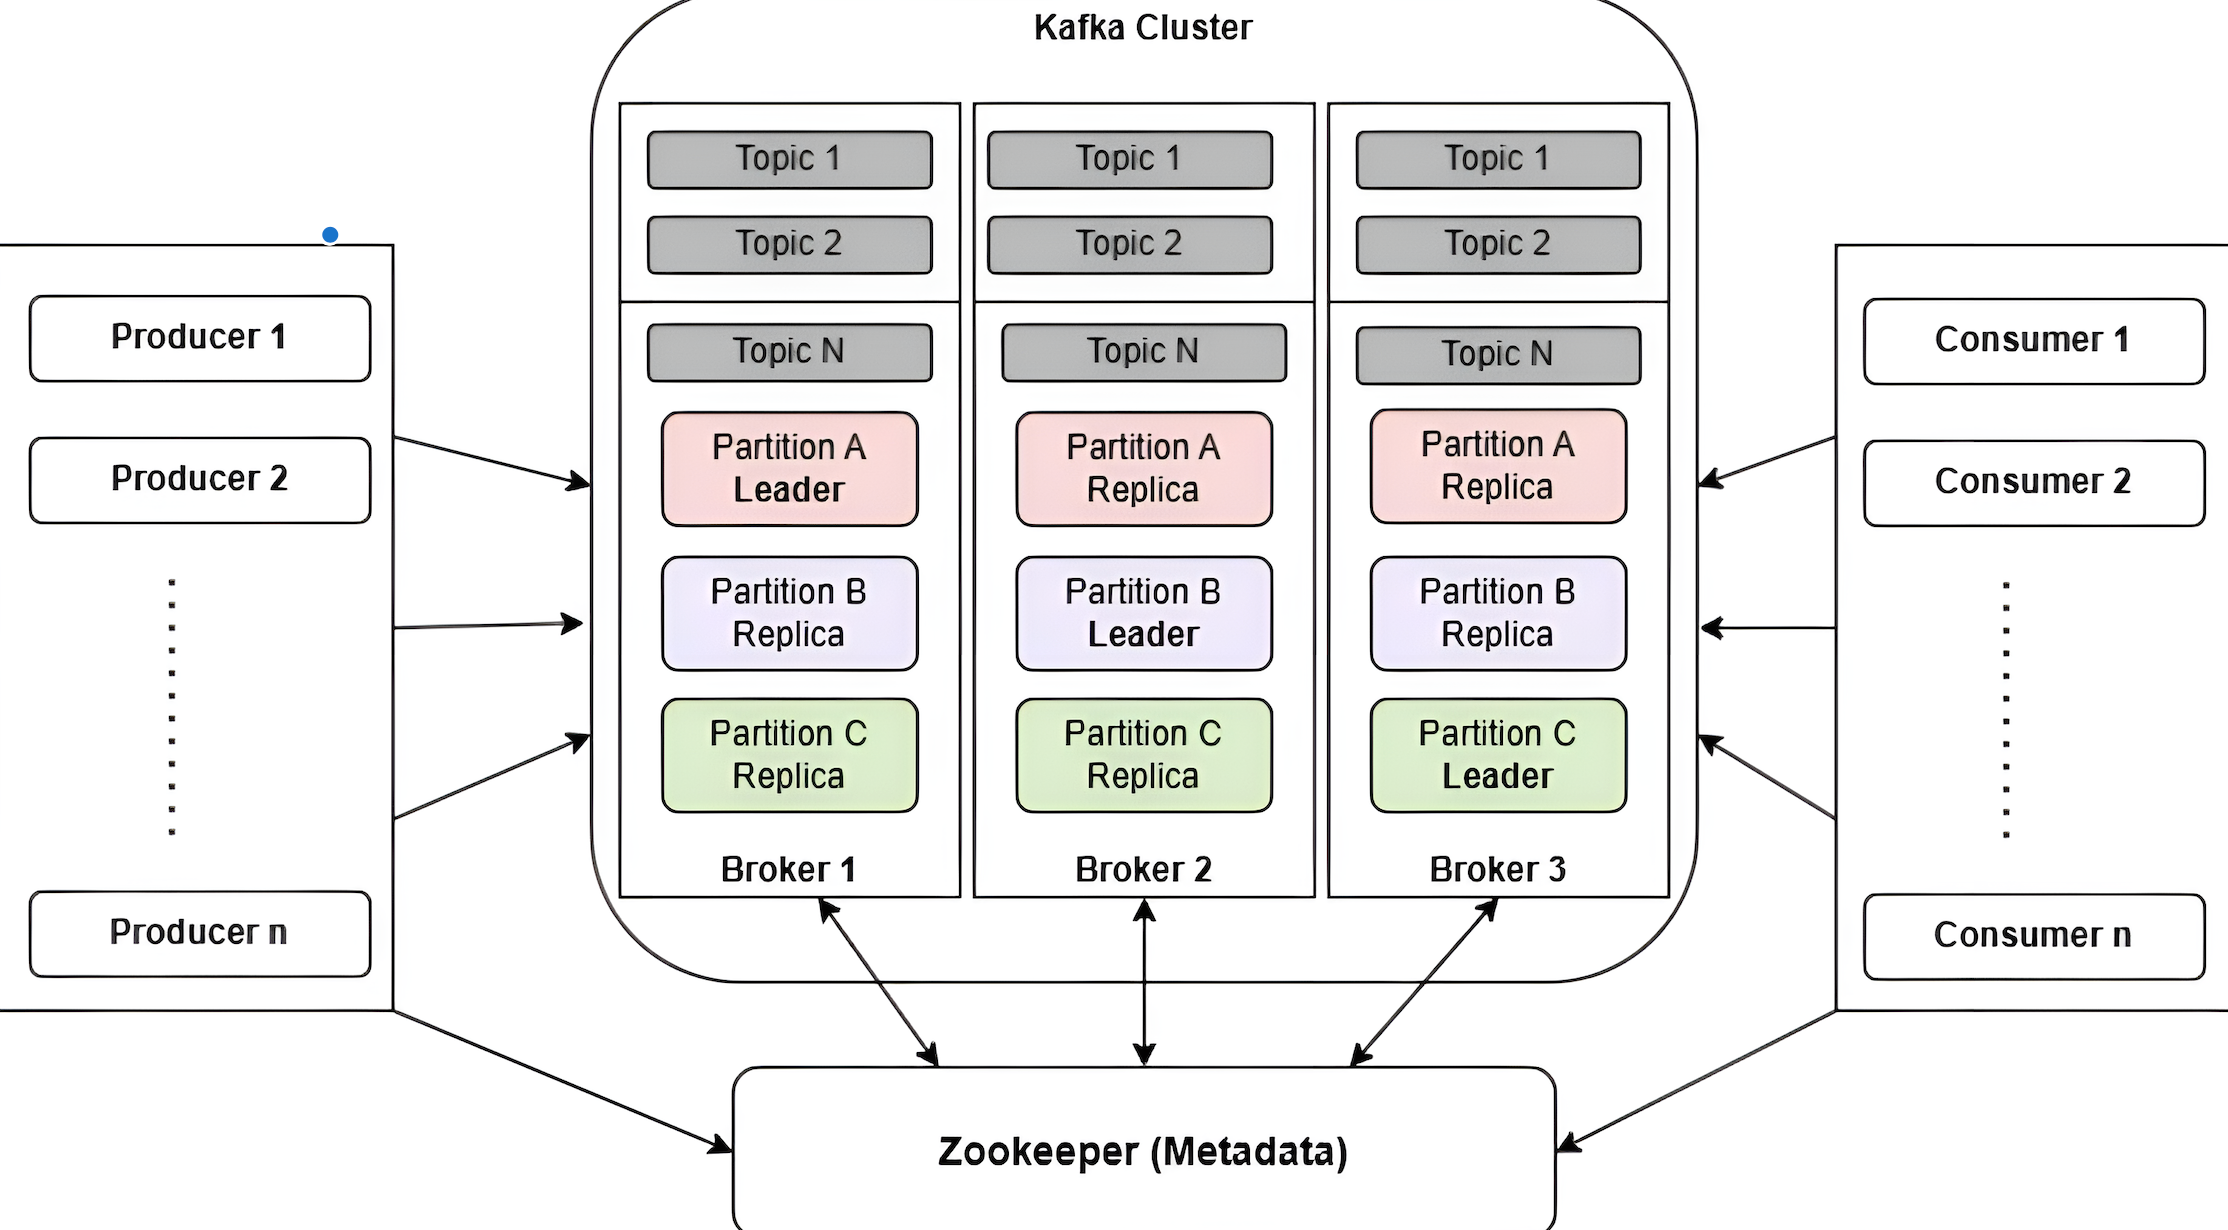
\includegraphics[width=1\textwidth]{Figure/kafka-fig.png}
    \caption{Kafka Architecture illustrating Producers, Consumers, Topics, Partitions, and Zookeeper \cite{whatiskafka}.}
    \label{fig:kafka_architecture}
\end{figure}

In Kafka's architecture, \textit{producers} generate data streams—such as encoded video frames in byte format, video metadata, and detected human bounding boxes—and send these streams to Kafka's storage system. In the context of person Re-ID, producers correspond to edge devices (e.g., surveillance cameras or edge processors). On the other hand, \textit{consumers} are processes initiated on central servers, which simultaneously subscribe to these data streams to retrieve and perform further processing, such as feature extraction, identity matching, and analytics. Kafka organizes these data streams into logical channels known as \textit{topics}, each representing a specific category or type of data. To enhance scalability, each topic is divided into multiple \textit{partitions}, enabling parallel processing and improved fault tolerance across distributed environments. 

This structured approach ensures Kafka can effectively manage data flow and scale seamlessly, making it particularly suited to complex, distributed Re-ID deployments.

\subsection{Model serving framework}
\label{sec:model_serving_framework}

Deploying person Re-ID and lightweight classification models effectively in hybrid edge–server architectures requires selecting an appropriate model-serving framework. Several well-known solutions such as TorchServe, TensorFlow Serving, and NVIDIA Triton Inference Server have been widely adopted. TorchServe~\cite{torchserve} is popular due to its native support and ease of use with PyTorch models, featuring straightforward REST APIs and dynamic batching to enhance GPU throughput. However, it lacks the ability to concurrently serve multiple instances of the same model efficiently on a single GPU, limiting maximal GPU utilization for lightweight models. TensorFlow Serving~\cite{tfserving}, while efficient in serving TensorFlow models, presents additional complexity for PyTorch-based workflows due to the necessity of model conversion. NVIDIA Triton Inference Server~\cite{triton}, meanwhile, excels at maximizing GPU usage through concurrent model execution and dynamic batching, enabling high throughput and efficient GPU resource allocation. Nevertheless, Triton's complexity and configuration overhead can present challenges, particularly for development teams prioritizing rapid deployment and ease of integration.

To balance these trade-offs, Ray Serve~\cite{ray_serve_docs} has emerged as an attractive framework, offering notable flexibility and ease of integration. Specifically designed for scalable deployments, Ray Serve supports serving multiple models simultaneously, dynamically composing inference pipelines, and efficiently managing replicas to maximize GPU utilization. Additionally, it seamlessly integrates with FastAPI, allowing developers to directly embed their inference endpoints within Python-based microservice architectures. This combination of flexible model orchestration, autoscaling capabilities, and developer-friendly integration makes Ray Serve particularly suited for deploying lightweight person Re-ID models like OSNet and LightMBN, as well as efficient image classification models, within hybrid edge–server setups.

\subsection{Containerization}
\label{sec:containerization}

Containerization is a foundational technology in modern DevOps and microservices architectures, enabling applications and their dependencies to be packaged into lightweight, isolated units. This approach simplifies development workflows and significantly improves service portability. By encapsulating services within containers, they can be deployed, scaled, and updated independently, which facilitates more efficient version control and lifecycle management in distributed systems.

Among the various container technologies, Docker \cite{docker_intro} is a widely used tool for building and running containers. Docker Engine serves as the core runtime that manages container lifecycle, including creation, execution, and resource allocation. Developers define application environments in a `Dockerfile`, which contains step-by-step instructions for building container images, including base operating system, dependencies, configuration files, and application code. This declarative approach ensures consistent behavior across both staging and production environments, eliminating the common "it works on my machine" problem. The Docker Engine utilizes Linux kernel features such as namespaces for process isolation and cgroups for resource management, enabling multiple containers to run securely on a single host without interference. Additionally, Docker's layered filesystem architecture allows for efficient image storage and sharing, where common layers are reused across different containers, reducing storage overhead and improving deployment speed.

\subsection{Vector Database}
\label{sec:vector_database}

Traditional databases, such as OLTP (Online Transaction Processing) and OLAP (Online Analytical Processing) systems, are optimized for structured queries and aggregated data operations. However, these systems typically face limitations when handling high-dimensional, continuous data like image feature embeddings. In contrast, \textbf{vector databases} are specifically designed to efficiently store and query vector representations, enabling rapid similarity searches based on distance metrics, notably cosine similarity.

Although widely used in Natural Language Processing (NLP) tasks like Retrieval-Augmented Generation (RAG), vector databases also significantly contribute to the person Re-ID domain by facilitating efficient identity matching. In person Re-ID systems, each individual's identity is stored as a high-dimensional feature vector—commonly 512 or 1024 dimensions—depending on the chosen deep learning feature extractor. During the retrieval stage, the system queries this vector database with a new feature vector to identify the most similar stored identities.

Several popular vector databases have emerged, each with distinct characteristics:

\begin{itemize}
  \item \textbf{Faiss}, developed by Meta, is a highly efficient C++ library offering both exact and approximate nearest-neighbor search using indexing strategies like Hierarchical Navigable Small World (HNSW), product quantization, and GPU acceleration~\cite{faiss}.
  
  \item \textbf{Milvus} is a scalable, distributed vector database built upon Faiss and hnswlib, supporting vast volumes of vectors and hybrid indexing methods optimized for distributed deployments~\cite{milvus}.
  
  \item \textbf{ChromaDB} is lightweight and optimized for NLP embeddings, providing simplicity and ease of use, though it may not offer the highest performance for large-scale or complex metadata queries~\cite{chromadb}.
  
  \item \textbf{Qdrant}, a Rust-based vector database, excels in hybrid queries due to its built-in support for efficient metadata filtering combined directly with vector search. Its HNSW indexing structure integrates metadata filtering during the search, significantly reducing query latency compared to post-filtering approaches~\cite{qdrant}.
  
  \item \textbf{Redis}, traditionally a key-value store, now includes vector search capabilities through the RediSearch module. Redis offers exceptional speed and convenience with its in-memory architecture, providing low-latency vector similarity searches while maintaining familiar Redis operations for metadata management. Its mature ecosystem and widespread adoption make it particularly attractive for hybrid edge-server deployments~\cite{redis_vector}.
  
  
\end{itemize}

Vector database indexes, such as HNSW \cite{hnsw}, differ fundamentally from traditional database indexes. Rather than focusing on exact matches or sorted queries, they organize vectors into graph-based structures optimized for approximate nearest-neighbor searches in high-dimensional spaces. The most commonly used distance metric in such scenarios is cosine similarity, which measures the angular similarity between vectors.

Among these alternatives, \textbf{Redis} emerges as the most suitable choice for our hybrid edge-server person Re-ID pipeline. Its in-memory architecture provides exceptional query performance, while its mature ecosystem and widespread adoption ensure reliable deployment and maintenance. Although Redis may have more limited advanced metadata filtering capabilities compared to specialized vector databases like Qdrant, its simplicity, speed, and integration convenience make it ideal for real-time person Re-ID applications where low latency is critical. Additionally, Redis's ability to handle both vector similarity searches and traditional key-value operations within a single system simplifies the overall architecture and reduces operational complexity.


\end{document}